\newpage
\section{Documento dei Requisiti}

\subsection{Raccolta dei requisiti}

\begin{itemize}
  \item[-] Per interagire con l’applicazione è necessario avere un utente registrato.
  \item[-] Per registrarsi l’utente deve inserire una mail univoca (Account), e una password lunga almeno 6 caratteri.
  \item[-] L’utente ha a disposizione un’agenda con gli eventi confermati e una con gli eventi proposti.
  \item[-] L’utente può creare un evento, definendo, al minimo, la data di inizio e di fine.
  \item[-] La data di fine deve essere successiva alla data di inizio.
  \item[-] L’utente può modificare un evento.
  \item[-] L’utente può confermare un evento condiviso, o disdire un evento confermato.
  \item[-] L’utente può condividere l’evento ad altri profili tramite link o condividendo a un gruppo o ad altri profili singoli.
  \item[-] L’utente può caricare le foto relative ad un evento, con visibilità condivisa.
  \item[-] Alla scadenza dell’evento, se su dispositivo mobile, l’applicazione controlla le foto scattate durante l’evento. Se ce ne sono, l’utente verrà notificato e potrà eliminare o confermare le foto, che verranno quindi caricate.
  \item[-] L’utente può cercare altri profili e creare un’associazione tra il profilo cercato e quello che sta usando.
  \item[-] I profili possono avere associazioni tra loro, a coppie o come gruppi.
  \item[-] L’utente può avere più profili, vedere in contemporanea gli eventi di tutti i profili associati ma effettuare le azioni a nome di uno solo.
  \item[-] La conferma/disdetta, il caricamento delle foto e la modifica di un evento deve avvenire in tempo reale se i profili condivisi sono online, altrimenti ricevono gli aggiornamenti all’avvio dell’applicazione.
  \item[-] L'applicazione deve essere intuitiva e con brevi tempi di risposta.
  \item[-] L'applicazione deve poter funzionare con un elevato numero di richieste concorrenti.
\end{itemize}


\subsection{Tabella dei Requisiti}

\begin{tabular} {|P{1.3cm}|P{11.2cm}|P{3cm}|}
  \hline
  \textbf{ID} & \textbf{Requisiti}                                                          & \textbf{Tipo}  \\
  \hline
  R1F         & Registrazione di un account tramite l’interfaccia web                       & Funzionale     \\
  \hline
  R2F         & Identificazione attraverso mail univoca e password di almeno 6 caratteri    & Funzionale     \\
  \hline
  R3F         & Visualizzazione degli eventi confermati                                     & Funzionale     \\
  \hline
  R4F         & Visualizzazione degli eventi proposti                                       & Funzionale     \\
  \hline
  R5F         & Creazione di un evento impostando almeno la data di inizio e quella di fine & Funzionale     \\
  \hline
  R6F         & La data di fine deve essere successiva alla data di inizio                  & Funzionale     \\
  \hline
  R7F         & Modifica di un evento                                                       & Funzionale     \\
  \hline
  R8F         & La conferma di un evento lo sposta negli eventi confermati                  & Funzionale     \\
  \hline
  R9F         & La disdetta di un evento lo sposta negli eventi proposti                    & Funzionale     \\
  \hline
  R10F        & Caricamento delle foto di un evento                                         & Funzionale     \\
  \hline
  R11F        & Condivisione tramite link                                                   & Funzionale     \\
  \hline
  R12F        & Condivisione tramite gruppo o ad altri profili                              & Funzionale     \\
  \hline
  R13F        & Ricerca automatica delle foto sul dispositivo mobile                        & Funzionale     \\
  \hline
  R14F        & Conferma delle foto                                                         & Funzionale     \\
  \hline
  R15F        & Ricerca di altri profili                                                    & Funzionale     \\
  \hline
  R16F        & Creazione di un gruppo da due o più profili                                 & Funzionale     \\
  \hline
  R17F        & Visualizzazione dei profili collegati                                       & Funzionale     \\
  \hline
  R18F        & Creazione di un nuovo profilo                                               & Funzionale     \\
  \hline
  R19F        & Cambio del profilo attualmente in uso                                       & Funzionale     \\
  \hline
  R20F        & Aggiornamento in tempo reale delle modifiche agli eventi                    & Funzionale     \\
  \hline
  R1NF        & Per interagire l’utente deve essere autenticato                             & Non Funzionale \\
  \hline
  R2NF        & Velocità di richiesta iniziale dei dati                                     & Non Funzionale \\
  \hline
  R3NF        & Semplicità e fluidità dell'interfaccia grafica                              & Non Funzionale \\
  \hline
  R4NF        & Velocità in lettura e scrittura dei dati                                    & Non Funzionale \\
  \hline
  R5NF        & Velocità nella ricerca dei profili                                          & Non Funzionale \\
  \hline
  R6NF        & Scalabilità delle richieste                                                 & Non Funzionale \\
  \hline
\end{tabular}
\clearpage

\subsection{Analisi dei Requisiti}
\subsubsection{Vocabolario}

\begin{tabular} {|P{3.5cm}|P{9cm}|P{3cm}|}
  \hline
  \textbf{Voce}     & \textbf{Definizione}                                                             & \textbf{Sinonimi}                 \\
  \hline
  Account           & combinazione di mail e password che identifica un utente                         &                                   \\
  \hline
  Utente            & Persona che utilizza l’applicazione                                              &                                   \\
  \hline
  Profilo           & Entità logica che raggruppa eventi e interazioni                                 &                                   \\
  \hline
  Profili collegati & Profili a cui l'utente può avere accesso                                         &                                   \\
  \hline
  Gruppo            & Insieme di profili                                                               &                                   \\
  \hline
  Evento            & Azione(o previsione di azione) con una durata nel tempo                          &                                   \\
  \hline
  Data e ora evento & Indicazione temporale del momento in cui avverrà l'azione                        &                                   \\
  \hline
  Evento confermato & Evento a cui il profilo ha dato conferma di partecipazione                       &                                   \\
  \hline
  Evento proposto   & Evento a cui il profilo non ha dato conferma di partecipazione                   & Evento disdetto, evento condiviso \\
  \hline
  Email             & Indirizzo di posta elettronica del cliente utilizzata anche per l'autenticazione &                                   \\
  \hline
  Password          & Codice alfanumerico di almeno 8 caratteri                                        &                                   \\
  \hline
  Credenziali       & Insieme composto da email e password necessari per accedere al sistema           &                                   \\
  \hline
\end{tabular}



\subsubsection{Sistemi esterni}
\label{sec:esterno}

Il sistema non dovrà interfacciarsi con sistemi esterni.


\newpage %optional
\subsubsection{Casi d'uso}

\begin{figure}[h!]
  \centering
    \adjustbox{valign=c, width=0.9\textheight, angle=90}{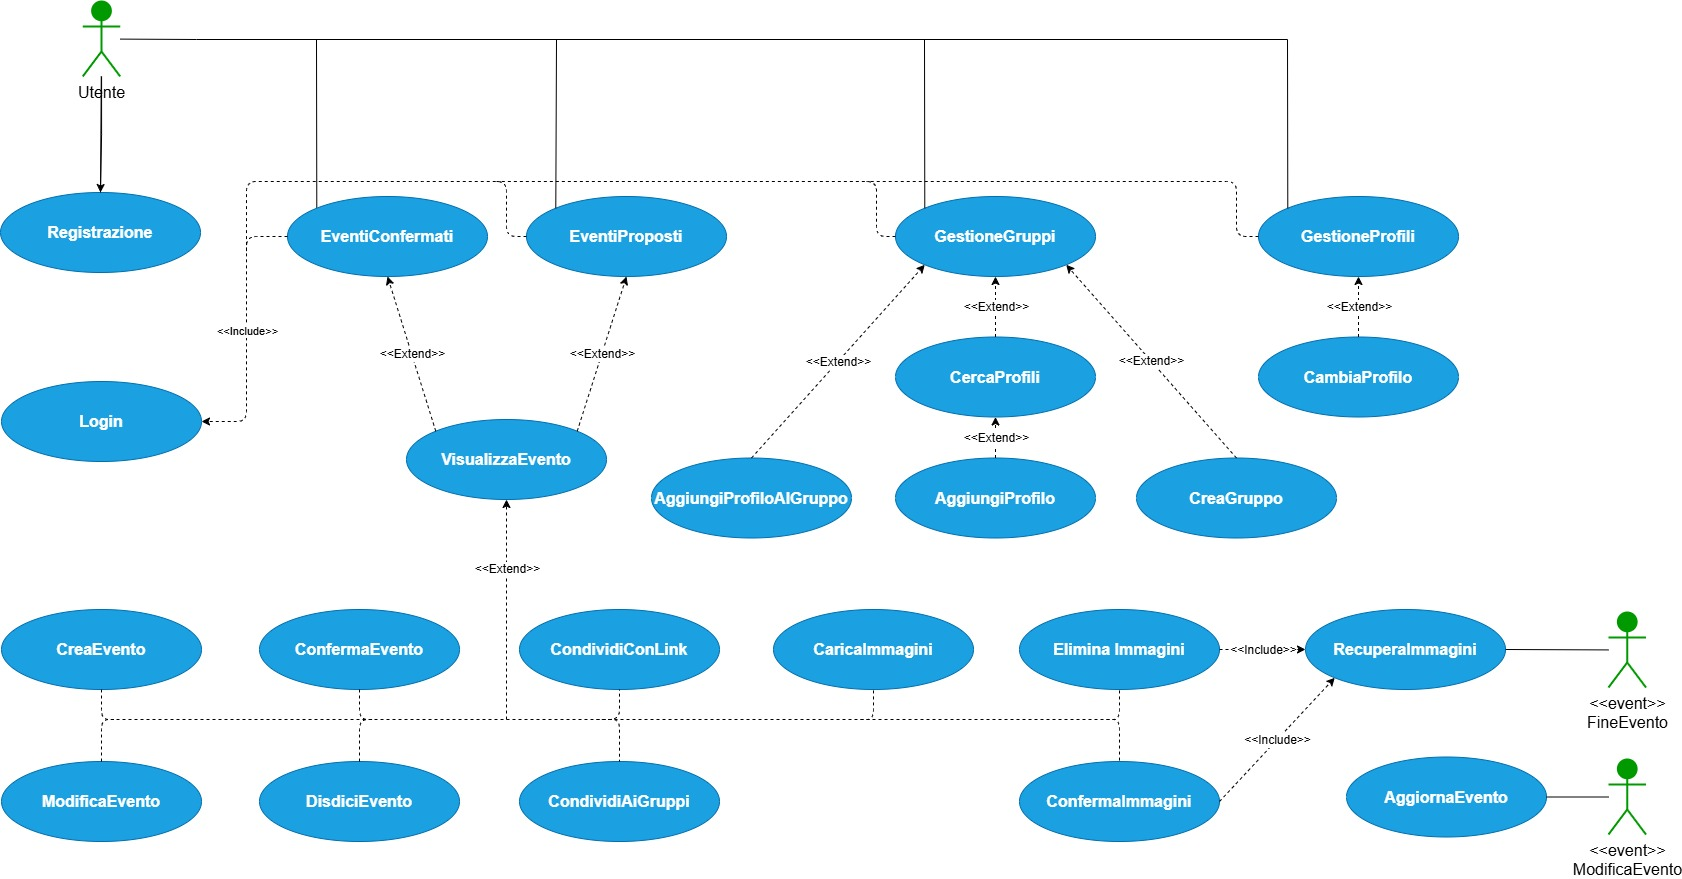
\includegraphics{Casiduso.jpg}}
\end{figure}

\newpage %optional
\subsubsection{Scenari}
\hfill \break

%Registrazione
\begin{tabular} {|P{4.5cm}|P{11cm}|}
  \hline
  \textbf{Titolo}                   & Registrazione                                                                            \\
  \hline
  \textbf{Descrizione}              & L'utente si registra al servizio                                                         \\
  \hline
  \textbf{Attori}                   & Utente                                                                                   \\
  \hline
  \textbf{Relazioni}                &                                                                                          \\
  \hline
  \textbf{Precondizioni}            &                                                                                          \\
  \hline
  \textbf{Postcondizioni}           & L'utente è registrato nel sistema e può interagire con il resto dell'applicazione        \\
  \hline
  \textbf{Scenario principale}      &
  1. L'utente accede alla sezione diregistrazione \linebreak
  2. L'utente inserisce email e  password \linebreak
  3. L'utente termina la registrazione, se avvenuta con successo viene reindirizzato alla pagina principale                    \\
  \hline
  \textbf{Scenari Alternativi}      &
  3. Il sistema verifica che è già presente un account con la mail inserita, quindi procede con la procedura di login normale. \\
  \hline
  \textbf{Requisiti non funzionali} &
  Per interagire l’utente deve essere autenticato \linebreak
  Velocità in lettura e scrittura dei dati                                                                                     \\
  \hline
  \textbf{Punti aperti}             &                                                                                          \\
  \hline
\end{tabular}
\hfill
\break

%Login
\begin{tabular} {|P{4.5cm}|P{11cm}|}
  \hline
  \textbf{Titolo}                   & Login                                                              \\
  \hline
  \textbf{Descrizione}              & Permette di accedere al sistema                                    \\
  \hline
  \textbf{Attori}                   & Utente                                                             \\
  \hline
  \textbf{Relazioni}                & EventiConfermati, EventiProposti, GestioneGruppi, GestioneProfili  \\
  \hline
  \textbf{Precondizioni}            &                                                                    \\
  \hline
  \textbf{Postcondizioni}           & L'utente ha accesso al sistema, limitato in base ai suoi privilegi \\
  \hline
  \textbf{Scenario principale}      & 1. L'utente inserisce le credenziali di
  accesso \linebreak 2. Il sistema verifica le credenziali \linebreak 3. Se le
  credenziali sono corrette, viene presentata la schermata iniziale                                      \\
  \hline
  \textbf{Scenari Alternativi}      & 1. L'utente inserisce le
  credenziali di accesso \linebreak 2. Il sistema verifica le credenziali
  \linebreak 3. Il sistema non riconosce le credenziali e rispedisce l'utente
  alla schermata di login con un messaggio di errore                                                     \\
  \hline
  \textbf{Requisiti non funzionali} & Velocità in lettura e scrittura dei dati\linebreak                 \\
  \hline
  \textbf{Punti aperti}             &                                                                    \\
  \hline
\end{tabular}
\hfill
\break

%EventiConfermati
\begin{tabular} {|P{4.5cm}|P{11cm}|}
  \hline
  \textbf{Titolo}                   & EventiConfermati                                            \\
  \hline
  \textbf{Descrizione}              & Viene mostrato l'elenco degli eventi confermati dall'utente \\
  \hline
  \textbf{Attori}                   & Utente                                                      \\
  \hline
  \textbf{Relazioni}                & Login, VisualizzaEvento                                     \\
  \hline
  \textbf{Precondizioni}            &                                                             \\
  \hline
  \textbf{Postcondizioni}           & Viene mostrato l'elenco degli eventi confermati             \\
  \hline
  \textbf{Scenario Principale}      & 1. L'utente va nella schermata di
  visualizzazione eventi confermati \linebreak 2. Il sistema recupera l'elenco degli eventi confermati \linebreak 3. Il sistema mostra a video
  l'elenco richiesto                                                                              \\
  \hline
  \textbf{Scenari Alternativi}      &                                                             \\
  \hline
  \textbf{Requisiti non funzionali} & Velocità di richiesta iniziale dei dati\linebreak
  Semplicità e fluidità dell'interfaccia grafica                                                  \\
  \hline
  \textbf{Punti aperti}             &                                                             \\
  \hline
\end{tabular}
\hfill
\break

%EventiProposti
\begin{tabular} {|P{4.5cm}|P{11cm}|}
  \hline
  \textbf{Titolo}                   & EventiProposti                                                           \\
  \hline
  \textbf{Descrizione}              & Viene mostrato l'elenco degli eventi proposti non confermati dall'utente \\
  \hline
  \textbf{Attori}                   & Utente                                                                   \\
  \hline
  \textbf{Relazioni}                & Login, VisualizzaEvento                                                  \\
  \hline
  \textbf{Precondizioni}            &                                                                          \\
  \hline
  \textbf{Postcondizioni}           & Viene mostrato l'elenco degli eventi proposti non confermati             \\
  \hline
  \textbf{Scenario Principale}      & 1. L'utente va nella schermata di
  visualizzazione eventi proposti \linebreak 2. Il sistema recupera l'elenco degli eventi proposti non confermati \linebreak 3. Il sistema mostra a video
  l'elenco richiesto                                                                                           \\
  \hline
  \textbf{Scenari Alternativi}      &                                                                          \\
  \hline
  \textbf{Requisiti non funzionali} & Velocità di richiesta iniziale dei dati\linebreak
  Semplicità e fluidità dell'interfaccia grafica                                                               \\
  \hline
  \textbf{Punti aperti}             &                                                                          \\
  \hline
\end{tabular}
\hfill
\break

%VisualizzaEvento
\begin{tabular} {|P{4.5cm}|P{11cm}|}
  \hline
  \textbf{Titolo}                   & VisualizzaEvento                                                                                                                                                                                   \\
  \hline
  \textbf{Descrizione}              & Viene mostrato l'evento con i suoi dettagli, con la possibilità di modificarli                                                                                                                     \\
  \hline
  \textbf{Attori}                   & Utente                                                                                                                                                                                             \\
  \hline
  \textbf{Relazioni}                & EventiConfermati, EventiProposti, CreaEvento, ModificaEvento, ConfermaEvento, DisdiciEvento, CondividiConLink, CondividiAiGruppi, CaricaImmagini, EliminaImmagini, ConfermaImmagini                \\
  \hline
  \textbf{Precondizioni}            &                                                                                                                                                                                                    \\
  \hline
  \textbf{Postcondizioni}           & Viene mostrato l'evento e i suoi dettagli, le modifiche vengono temporaneamente salvate                                                                                                            \\
  \hline
  \textbf{Scenario Principale}      & 1. L'utente seleziona un evento \linebreak 2. Il sistema recupera i dati dell'evento \linebreak 3. Il sistema mostra a video i dati dell'evento da la possibilità di modificare i dati dell'evento \\
  \hline
  \textbf{Scenari Alternativi}      & Scenario alternativo A: \linebreak
  1. L'utente seleziona l'opzione di creare un nuovo evento \linebreak 2. Il sistema mostra a video i dati dell'evento da la possibilità di modificare i dati dell'evento         \linebreak
  Scenario alternativo B:\linebreak
  1. L'utente viene indirizzato tramite link\linebreak
  2. Il sistema recupera i dati dell'evento\linebreak
  3. Il sistema mostra a video i dati dell'evento da la possibilità di modificare i dati dell'evento                                                                                                                                     \\
  \hline
  \textbf{Requisiti non funzionali} & Velocità in lettura e scrittura dei dati\linebreak
  Semplicità e fluidità dell'interfaccia grafica                                                                                                                                                                                         \\
  \hline
  \textbf{Punti aperti}             &                                                                                                                                                                                                    \\
  \hline
\end{tabular}
\hfill
\break

%CreaEvento
\begin{tabular} {|P{4.5cm}|P{11cm}|}
  \hline
  \textbf{Titolo}                   & CreaEvento                                                                        \\
  \hline
  \textbf{Descrizione}              & Crea un evento e lo aggiunge                                                      \\
  \hline
  \textbf{Attori}                   & Utente                                                                            \\
  \hline
  \textbf{Relazioni}                & VisualizzaEvento                                                                  \\
  \hline
  \textbf{Precondizioni}            & L'evento non esiste, i dati inseriti sono corretti                                \\
  \hline
  \textbf{Postcondizioni}           & Viene creato l'evento e visualizzato nella pagina relativa                        \\
  \hline
  \textbf{Scenario Principale}      & 1. VisualizzaEvento \linebreak
  2. Il sistema controlla che i dati inseriti siano corretti\linebreak
  3. Se i dati sono corretti, l'evento viene salvato\linebreak
  4. L'evento è visualizzato nella schermata degli eventi\linebreak
  5. Tutti i dispositivi collegati al profilo visualizzano l'evento                                                     \\
  \hline
  \textbf{Scenari Alternativi}      & 3. Se i dati risultano sbagliati, il sistema notifica l'utente indicando l'errore \\
  \hline
  \textbf{Requisiti non funzionali} & Velocità in lettura e scrittura dei dati                                          \\
  \hline
  \textbf{Punti aperti}             &                                                                                   \\
  \hline
\end{tabular}
\hfill
\break

%ModificaEvento
\begin{tabular} {|P{4.5cm}|P{11cm}|}
  \hline
  \textbf{Titolo}                   & ModificaEvento                                                                    \\
  \hline
  \textbf{Descrizione}              & Salva le modifiche ad un evento                                                   \\
  \hline
  \textbf{Attori}                   & Utente                                                                            \\
  \hline
  \textbf{Relazioni}                & VisualizzaEvento                                                                  \\
  \hline
  \textbf{Precondizioni}            & L'evento esiste e sono stati modificati dei dati                                  \\
  \hline
  \textbf{Postcondizioni}           & Le modifiche vengono salvate e propagate a tutti i profili collegati              \\
  \hline
  \textbf{Scenario Principale}      & 1. VisualizzaEvento \linebreak
  2. Il sistema controlla che i dati modificati siano corretti\linebreak
  3. Le immagini vengono salvate\linebreak
  4. Tutti i dispositivi collegati ai profili collegati all'evento visualizzano le immagini                             \\
  \hline
  \textbf{Scenari Alternativi}      & 3. Se i dati risultano sbagliati, il sistema notifica l'utente indicando l'errore \\
  \hline
  \textbf{Requisiti non funzionali} & Velocità in lettura e scrittura dei dati                                          \\
  \hline
  \textbf{Punti aperti}             &                                                                                   \\
  \hline
\end{tabular}
\hfill
\break

%ConfermaEvento
\begin{tabular} {|P{4.5cm}|P{11cm}|}
  \hline
  \textbf{Titolo}                   & ConfermaEvento                                                                                                                       \\
  \hline
  \textbf{Descrizione}              & Conferma la partecipazione ad un evento                                                                                              \\
  \hline
  \textbf{Attori}                   & Utente                                                                                                                               \\
  \hline
  \textbf{Relazioni}                & VisualizzaEvento                                                                                                                     \\
  \hline
  \textbf{Precondizioni}            & L'evento esiste e il profilo corrente non lo ha confermato                                                                           \\
  \hline
  \textbf{Postcondizioni}           & Il profilo conferma la sua presenza, tutti i profili collegati vengono aggiornati, l'evento è visualizzato tra gli eventi confermati \\
  \hline
  \textbf{Scenario Principale}      & 1. VisualizzaEvento \linebreak
  2. L'utente conferma la sua presenza\linebreak
  3. L'evento è visualizzato tra gli eventi confermati\linebreak
  4. Tutti i dispositivi collegati ai profili collegati all'evento visualizzano l'aggiornamento                                                                            \\
  \hline
  \textbf{Scenari Alternativi}      &                                                                                                                                      \\
  \hline
  \textbf{Requisiti non funzionali} & Velocità in lettura e scrittura dei dati                                                                                             \\
  \hline
  \textbf{Punti aperti}             &                                                                                                                                      \\
  \hline
\end{tabular}
\hfill
\break

%DisdiciEvento
\begin{tabular} {|P{4.5cm}|P{11cm}|}
  \hline
  \textbf{Titolo}                   & DisdiciEvento                                                                                                                     \\
  \hline
  \textbf{Descrizione}              & Disdice la partecipazione ad un evento                                                                                            \\
  \hline
  \textbf{Attori}                   & Utente                                                                                                                            \\
  \hline
  \textbf{Relazioni}                & VisualizzaEvento                                                                                                                  \\
  \hline
  \textbf{Precondizioni}            & L'evento esiste e il profilo corrente lo ha confermato                                                                            \\
  \hline
  \textbf{Postcondizioni}           & Il profilo disdice la sua presenza, tutti i profili collegati vengono aggiornati, l'evento è visualizzato tra gli eventi proposti \\
  \hline
  \textbf{Scenario Principale}      & 1. VisualizzaEvento \linebreak
  2. L'utente disdice la sua presenza\linebreak
  3. L'evento è visualizzato tra gli eventi proposti\linebreak
  4. Tutti i dispositivi collegati ai profili collegati all'evento visualizzano l'aggiornamento                                                                         \\
  \hline
  \textbf{Scenari Alternativi}      &                                                                                                                                   \\
  \hline
  \textbf{Requisiti non funzionali} & Velocità in lettura e scrittura dei dati                                                                                          \\
  \hline
  \textbf{Punti aperti}             &                                                                                                                                   \\
  \hline
\end{tabular}
\hfill
\break

%CaricaImmagini
\begin{tabular} {|P{4.5cm}|P{11cm}|}
  \hline
  \textbf{Titolo}                   & CaricaImmagini                                                                  \\
  \hline
  \textbf{Descrizione}              & Permette all'utente di selezionare immagini da collegare all'evento, salvandole \\
  \hline
  \textbf{Attori}                   & Utente                                                                          \\
  \hline
  \textbf{Relazioni}                & VisualizzaEvento                                                                \\
  \hline
  \textbf{Precondizioni}            & L'evento esiste                                                                 \\
  \hline
  \textbf{Postcondizioni}           & Le immagini vengono salvate e propagate a tutti i profili collegati             \\
  \hline
  \textbf{Scenario Principale}      & 1. VisualizzaEvento \linebreak
  2. L'utente seleziona le immagini che vuole caricare\linebreak
  3. Le immagini vengono salvate\linebreak
  4. Tutti i dispositivi collegati ai profili collegati all'evento visualizzano le immagini                           \\
  \hline
  \textbf{Scenari Alternativi}      &                                                                                 \\
  \hline
  \textbf{Requisiti non funzionali} & Velocità in lettura e scrittura dei dati\linebreak
  Semplicità e fluidità dell'interfaccia grafica                                                                      \\
  \hline
  \textbf{Punti aperti}             &                                                                                 \\
  \hline
\end{tabular}
\hfill
\break

%RecuperaImmagini
\begin{tabular} {|P{4.5cm}|P{11cm}|}
  \hline
  \textbf{Titolo}                   & RecuperaImmagini                                                          \\
  \hline
  \textbf{Descrizione}              & Controlla la galleria e salva in locale le foto scattate durante l'evento \\
  \hline
  \textbf{Attori}                   & FineEvento                                                                \\
  \hline
  \textbf{Relazioni}                & EliminaImmagini, ConfermaImmagini                                         \\
  \hline
  \textbf{Precondizioni}            & L'evento esiste ed è concluso                                             \\
  \hline
  \textbf{Postcondizioni}           & Le immagini vengono salvate in locale e l'utente viene notificato         \\
  \hline
  \textbf{Scenario Principale}      & 1. Il sistema controlla che l'evento sia finito \linebreak
  2. Il sistema controlla la galleria per trovare le immagini scattate nell'arco temporale dell'evento\linebreak
  3. Se ci sono immagini, vengono salvate in locale e l'utente viene notificato                                 \\
  \hline
  \textbf{Scenari Alternativi}      &                                                                           \\
  \hline
  \textbf{Requisiti non funzionali} & Velocità in lettura e scrittura dei dati                                  \\
  \hline
  \textbf{Punti aperti}             &                                                                           \\
  \hline
\end{tabular}
\hfill
\break

%EliminaImmagini
\begin{tabular} {|P{4.5cm}|P{11cm}|}
  \hline
  \textbf{Titolo}                   & EliminaImmagini                                       \\
  \hline
  \textbf{Descrizione}              & Rimuove le immagini dall'evento                       \\
  \hline
  \textbf{Attori}                   & Utente                                                \\
  \hline
  \textbf{Relazioni}                & RecuperaImmagini, VisualizzaEvento                    \\
  \hline
  \textbf{Precondizioni}            & L'evento esiste ed esistono immagini collegate        \\
  \hline
  \textbf{Postcondizioni}           & Le immagini selezionate vengono rimosse dall'evento   \\
  \hline
  \textbf{Scenario Principale}      & 1.VisualizzaEvento
  1. L'utente seleziona le immagini caricate automaticamente da eliminare\linebreak
  1. Le immagini vengono rimosse dall'evento                                                \\
  \hline
  \textbf{Scenari Alternativi}      & 1. VisualizzaEvento \linebreak
  2. L'utente seleziona le immagini da eliminare\linebreak
  3. Le immagini vengono rimosse dall'evento, e le modifiche propagate ai profili collegati \\
  \hline
  \textbf{Requisiti non funzionali} &                                                       \\
  \hline
  \textbf{Punti aperti}             &                                                       \\
  \hline
\end{tabular}
\hfill
\break

%ConfermaImmagini
\begin{tabular} {|P{4.5cm}|P{11cm}|}
  \hline
  \textbf{Titolo}                   & ConfermaImmagini                                              \\
  \hline
  \textbf{Descrizione}              & L'utente conferma le immagini caricate automaticamente        \\
  \hline
  \textbf{Attori}                   & Utente                                                        \\
  \hline
  \textbf{Relazioni}                & RecuperaImmagini, VisualizzaEvento                            \\
  \hline
  \textbf{Precondizioni}            & L'evento esiste ed esistono immagini caricate automaticamente \\
  \hline
  \textbf{Postcondizioni}           & Le immagini selezionate vengono condivise con l'evento        \\
  \hline
  \textbf{Scenario Principale}      & 1. VisualizzaEvento \linebreak
  2. L'utente seleziona conferma le immagini caricate automaticamente\linebreak
  3. Le immagini vengono aggiunte all'evento e tutti i profili collegati visualizzano le modifiche  \\
  \hline
  \textbf{Scenari Alternativi}      &                                                               \\
  \hline
  \textbf{Requisiti non funzionali} & Velocità in lettura e scrittura dei dati                      \\
  \hline
  \textbf{Punti aperti}             &                                                               \\
  \hline
\end{tabular}
\hfill
\break

%CondividiAiGruppi
\begin{tabular} {|P{4.5cm}|P{11cm}|}
  \hline
  \textbf{Titolo}                   & CondividiAiGruppi                                                           \\
  \hline
  \textbf{Descrizione}              & Permette di condividere l'evento ai gruppi                                  \\
  \hline
  \textbf{Attori}                   & Utente                                                                      \\
  \hline
  \textbf{Relazioni}                & VisualizzaEvento                                                            \\
  \hline
  \textbf{Precondizioni}            & L'evento esiste                                                             \\
  \hline
  \textbf{Postcondizioni}           & L'evento è condiviso con tutti i profili appartenenti ai gruppi selezionati \\
  \hline
  \textbf{Scenario Principale}      & 1. VisualizzaEvento\linebreak
  2. Il sistema visualizza l'elenco dei gruppi di cui l'utente fa parte, permettendone la selezione\linebreak
  3. L'evento è condiviso con tutti i profili dei gruppi selezionati, che visualizzeranno l'evento tra i proposti \\
  \hline
  \textbf{Scenari Alternativi}      &                                                                             \\
  \hline
  \textbf{Requisiti non funzionali} & Velocità in lettura e scrittura dei dati                                    \\
  \hline
  \textbf{Punti aperti}             &                                                                             \\
  \hline
\end{tabular}
\hfill
\break

%CondividiConLink
\begin{tabular} {|P{4.5cm}|P{11cm}|}
  \hline
  \textbf{Titolo}                   & CondividiConLink                                  \\
  \hline
  \textbf{Descrizione}              & Permette di condividere l'evento tramite link     \\
  \hline
  \textbf{Attori}                   & Utente                                            \\
  \hline
  \textbf{Relazioni}                & VisualizzaEvento                                  \\
  \hline
  \textbf{Precondizioni}            & L'evento esiste                                   \\
  \hline
  \textbf{Postcondizioni}           & L'utente ottiene un link che può confidividere    \\
  \hline
  \textbf{Scenario Principale}      & 1. VisualizzaEvento\linebreak
  2. Il sistema mostra le opzioni di condivisione del link                              \\
  \hline
  \textbf{Scenari Alternativi}      & 2. Il sistema salva il link in memoria temporanea \\
  \hline
  \textbf{Requisiti non funzionali} & Velocità in lettura e scrittura dei dati          \\
  \hline
  \textbf{Punti aperti}             &                                                   \\
  \hline
\end{tabular}
\hfill
\break

%AggiornaEvento
\begin{tabular} {|P{4.5cm}|P{11cm}|}
  \hline
  \textbf{Titolo}                   & AggiornaEvento                                                                  \\
  \hline
  \textbf{Descrizione}              & Aggiorna l’evento in locale in base alle modifiche apportate da profili esterni \\
  \hline
  \textbf{Attori}                   & ModificaEvento                                                                  \\
  \hline
  \textbf{Relazioni}                &                                                                                 \\
  \hline
  \textbf{Precondizioni}            & L'evento esiste ed è cdondiviso con uno dei profili collegati all'utente        \\
  \hline
  \textbf{Postcondizioni}           & L'evento viene aggiornato con le modifiche                                      \\
  \hline
  \textbf{Scenario Principale}      & 1. Il sistema riceve la notifica che un evento è stato modificato \linebreak
  2. Il sistema recupera le modifiche e aggiorna l'evento di conseguenza                                              \\
  \hline
  \textbf{Scenari Alternativi}      &                                                                                 \\
  \hline
  \textbf{Requisiti non funzionali} & Velocità in lettura e scrittura dei dati\                                       \\
  \hline
  \textbf{Punti aperti}             &                                                                                 \\
  \hline
\end{tabular}
\hfill
\break

%GestioneGruppi
\begin{tabular} {|P{4.5cm}|P{11cm}|}
  \hline
  \textbf{Titolo}                   & GestioneGruppi                                                        \\
  \hline
  \textbf{Descrizione}              & Viene mostrato l'elenco dei gruppi appartenenti al profilo corrente   \\
  \hline
  \textbf{Attori}                   & Utente                                                                \\
  \hline
  \textbf{Relazioni}                & Login, CercaProfili, CreaGruppo                                       \\
  \hline
  \textbf{Precondizioni}            &                                                                       \\
  \hline
  \textbf{Postcondizioni}           & Viene mostrato l'elenco degli gruppi appartenenti al profilo corrente \\
  \hline
  \textbf{Scenario Principale}      & 1. L'utente va nella schermata di gestione gruppi \linebreak
  2. Il sistema recupera l'elenco dei gruppi appartenenti al profilo corrente \linebreak
  3. Il sistema mostra a video l'elenco richiesto                                                           \\
  \hline
  \textbf{Scenari Alternativi}      &                                                                       \\
  \hline
  \textbf{Requisiti non funzionali} & Velocità di richiesta iniziale dei dati\linebreak
  Semplicità e fluidità dell'interfaccia grafica                                                            \\
  \hline
  \textbf{Punti aperti}             &                                                                       \\
  \hline
\end{tabular}
\hfill
\break

%CercaProfili
\begin{tabular} {|P{4.5cm}|P{11cm}|}
  \hline
  \textbf{Titolo}                   & CercaProfili                                              \\
  \hline
  \textbf{Descrizione}              & L'utente cerca i profili tramite tag                      \\
  \hline
  \textbf{Attori}                   & Utente                                                    \\
  \hline
  \textbf{Relazioni}                & GestioneGruppi, AggiungiProfilo                           \\
  \hline
  \textbf{Precondizioni}            &                                                           \\
  \hline
  \textbf{Postcondizioni}           & Si visualizza la lista dei profili con tag corrispondente \\
  \hline
  \textbf{Scenario principale}      & 1. GestioneGruppi \linebreak
  2. L'utente inserisce il tag parziale o completo del profilo per cui eseguire la ricerca \linebreak
  3. Il sistema ottiene la lista dei profili che corrispondono alla ricerca\linebreak
  4. La lista viene mostrata all'utente                                                         \\
  \hline
  \textbf{Scenari Alternativi}      &                                                           \\
  \hline
  \textbf{Requisiti non funzionali} & Velocità in lettura e scrittura dei dati\linebreak
  Semplicità e fluidità dell'interfaccia grafica                                                \\
  \hline
  \textbf{Punti aperti}             &                                                           \\
  \hline
\end{tabular}
\hfill
\break

%AggiungiProfilo
\begin{tabular} {|P{4.5cm}|P{11cm}|}
  \hline
  \textbf{Titolo}                   & AggiungiProfilo                                                  \\
  \hline
  \textbf{Descrizione}              & si aggiunge il profilo selezionato alla lista gruppi del profilo \\
  \hline
  \textbf{Attori}                   & Utente                                                           \\
  \hline
  \textbf{Relazioni}                & CercaProfili                                                     \\
  \hline
  \textbf{Precondizioni}            & Il profilo selezionato esiste                                    \\
  \hline
  \textbf{Postcondizioni}           & Il profilo selezionato è visibile tra la lista dei gruppi        \\
  \hline
  \textbf{Scenario principale}      & 1. CercaProfili \linebreak
  2. L'utente seleziona il profilo da aggiungere \linebreak
  3. Il profilo viene aggiunto nella lista dei gruppi\linebreak                                        \\
  \hline
  \textbf{Scenari Alternativi}      &                                                                  \\
  \hline
  \textbf{Requisiti non funzionali} & Velocità in lettura e scrittura dei dati                         \\
  \hline
  \textbf{Punti aperti}             &                                                                  \\
  \hline
\end{tabular}
\hfill
\break

%CreaGruppo
\begin{tabular} {|P{4.5cm}|P{11cm}|}
  \hline
  \textbf{Titolo}                   & CreaGruppo                                                                          \\
  \hline
  \textbf{Descrizione}              & L'utente crea un gruppo                                                             \\
  \hline
  \textbf{Attori}                   & Utente                                                                              \\
  \hline
  \textbf{Relazioni}                & GestioneGruppi, AggiungiProfiloAlGruppo                                             \\
  \hline
  \textbf{Precondizioni}            &                                                                                     \\
  \hline
  \textbf{Postcondizioni}           & Il gruppo è creato ed aggiunto alla lista dei gruppi di tutti i profili interessati \\
  \hline
  \textbf{Scenario principale}      & 1. GestioneGruppi \linebreak
  2. L'utente inserisce il nome ed eventualmente i profili interessati \linebreak
  3. Il sistema crea il gruppo e lo aggiunge alla lista dei gruppi di tutti i profili interessati\linebreak               \\
  \hline
  \textbf{Scenari Alternativi}      &                                                                                     \\
  \hline
  \textbf{Requisiti non funzionali} & Velocità in lettura e scrittura dei dati                                            \\
  \hline
  \textbf{Punti aperti}             &                                                                                     \\
  \hline
\end{tabular}
\hfill
\break

%AggiungiProfiloAlGruppo
\begin{tabular} {|P{4.5cm}|P{11cm}|}
  \hline
  \textbf{Titolo}                   & AggiungiProfiloAlGruppo                                          \\
  \hline
  \textbf{Descrizione}              & si aggiunge il profilo selezionato alla lista gruppi del profilo \\
  \hline
  \textbf{Attori}                   & Utente                                                           \\
  \hline
  \textbf{Relazioni}                & GestioneGruppi                                                   \\
  \hline
  \textbf{Precondizioni}            & Il profilo selezionato esiste                                    \\
  \hline
  \textbf{Postcondizioni}           & Il profilo selezionato è tra la lista i profili del gruppo       \\
  \hline
  \textbf{Scenario principale}      & 1. GestioneGruppi \linebreak
  2. L'utente seleziona il profilo da aggiungere\linebreak
  3. Il sistema aggiunge il profilo alla lista dei profili del gruppo\linebreak
  4. Il profilo aggiunto visualizza il gruppo nella sua lista dei gruppi                               \\
  \hline
  \textbf{Scenari Alternativi}      &                                                                  \\
  \hline
  \textbf{Requisiti non funzionali} & Velocità in lettura e scrittura dei dati                         \\
  \hline
  \textbf{Punti aperti}             &                                                                  \\
  \hline
\end{tabular}
\hfill
\break

%GestioneProfili
\begin{tabular} {|P{4.5cm}|P{11cm}|}
  \hline
  \textbf{Titolo}                   & GestioneProfili                                               \\
  \hline
  \textbf{Descrizione}              & Viene mostrato l'elenco dei profili collegati all'utente      \\
  \hline
  \textbf{Attori}                   & Utente                                                        \\
  \hline
  \textbf{Relazioni}                & Login, CambiaProfilo                                          \\
  \hline
  \textbf{Precondizioni}            &                                                               \\
  \hline
  \textbf{Postcondizioni}           & Viene mostrato l'elenco degli profili collegati all'utente    \\
  \hline
  \textbf{Scenario Principale}      & 1. L'utente va nella schermata di gestione profili \linebreak
  2. Il sistema recupera l'elenco dei profili collegati all'utente \linebreak
  3. Il sistema mostra a video l'elenco richiesto                                                   \\
  \hline
  \textbf{Scenari Alternativi}      &                                                               \\
  \hline
  \textbf{Requisiti non funzionali} & Velocità di richiesta iniziale dei dati\linebreak
  Semplicità e fluidità dell'interfaccia grafica                                                    \\
  \hline
  \textbf{Punti aperti}             &                                                               \\
  \hline
\end{tabular}
\hfill
\break

%CambiaProfilo
\begin{tabular} {|P{4.5cm}|P{11cm}|}
  \hline
  \textbf{Titolo}                   & CambiaProfilo                                            \\
  \hline
  \textbf{Descrizione}              & Modifica il profilo corrente con quello selezionato      \\
  \hline
  \textbf{Attori}                   & Utente                                                   \\
  \hline
  \textbf{Relazioni}                & GestioneProfili                                          \\
  \hline
  \textbf{Precondizioni}            & Il profilo selezionabile non è quello attualmente in uso \\
  \hline
  \textbf{Postcondizioni}           & Il profilo corrente è quello che è stato selezionato     \\
  \hline
  \textbf{Scenario Principale}      & 1. GestioneProfili \linebreak
  2. L'utente seleziona il profilo\linebreak
  3. Il profilo corrente diventa quello selezionato                                            \\
  \hline
  \textbf{Scenari Alternativi}      &                                                          \\
  \hline
  \textbf{Requisiti non funzionali} &                                                          \\
  \hline
  \textbf{Punti aperti}             &                                                          \\
  \hline
\end{tabular}
\hfill
\break

\subsection{Analisi del Rischio}

\subsubsection{Tabella Valutazione dei Beni}

\begin{tabular} {|P{3.5cm}|P{5.5cm}|P{6.7cm}|}
  \hline
  \textbf{Bene}                     & \textbf{Valore}                                                                                              & \textbf{Esposizione}      \\
  \hline
  Sistema Informativo               & Alto. Fondamentale per il funzionamento del servizio                                                         &
  Alta. Perdita finanziaria e di immagine                                                                                                                                      \\
  \hline
  Informazioni dei clienti          & Alto. Informazioni personali                                                                                 &
  Alta. Perdita di immagine dovuta alla divulgazione
  di dati sensibili                                                                                                                                                            \\
  \hline
  Informazioni relativi agli eventi & Medio-alto, necessari per offrire il servizio e contenenti informazioni personali e potenzialmente riservate &
  Molto Alta. Perdita di immagine possibile con la divulgazione dei dati relativi ai
  clienti                                                                                                                                                                      \\
  \hline
  Dati dei gruppi                   & Medio. Necessario per condividere gli eventi                                                                 & Alta. Perdita di immagine \\
  \hline
\end{tabular}

\subsubsection{Tabella Minacce/Controlli}

\begin{tabular} {|P{3cm}|P{2cm}|P{6.1cm}|P{4cm}|}
  \hline
  \textbf{Minaccia}                                 & \textbf{Probab.} & \textbf{Controllo}                                                                                                                                                                                                                      & \textbf{Fattibilità}                                              \\
  \hline
  Furto credenziali utente                          & Alta             & Controllo sulla sicurezza della password - Log delle operazioni, autenticazione a due fattori                                                                                                                                           & Costo implementativo medio                                        \\
  \hline
  Alterazione o intercettazione delle comunicazioni & Alta             & Utilizzo di un canale sicuro - Log delle operazioni, autenticazione integrata nel messaggio                                                                                                                                             & Basso costo di realizzazione con determinati protocolli           \\
  \hline
  Accesso non autorizzato al database               & Bassa            & Accesso da macchine sicure - Log di tutte le operazioni                                                                                                                                                                                 & Basso costo di realizzazione, il server deve essere ben custodito \\
  \hline
  DoS                                               & Bassa            & Controllo e limitazione delle richieste                                                                                                                                                                                                 & Media complessità di implementazione                              \\
  \hline
  Saturazione del database                          & Bassa            & 1. Limitazione delle richieste in un dato intervallo di tempo. \linebreak 2. Limitazione della grandezza delle richieste singole \linebreak 3. Limitazione della grandezza richiesta dallo stesso utente in un dato intervallo di tempo & Media complessità di implementazione                              \\
  \hline
\end{tabular}

\subsubsection{Analisi Tecnologica della Sicurezza}

\begin{tabular} {|P{4cm}|P{12cm}|}
  \hline
  Tecnologia                     & Vulnerabilità                                            \\
  \hline
  Autenticazione email/password  & • Utente rivela volontariamente la password \linebreak
  • Utente rivela la password con un attacco di ingegneria sociale \linebreak
  • Password banali                                                                         \\
  \hline
  Cifratura comunicazioni        & • In caso di cifratura simmetrica particolare
  attenzione va alla lunghezza delle chiavi ed alla loro memorizzazione                     \\
  \hline
  Architettura Client/Server     & • DoS \linebreak
  • Man in the Middle \linebreak
  • Sniffing delle comunicazioni                                                            \\
  \hline
  Connessione Server/Persistenza & • Limite massimo di connessioni contemporanee \linebreak
  • Saturazione del Database                                                                \\
  \hline
\end{tabular}

\newpage
\subsubsection{Security Use Case \& Misuse Case}
\par

\begin{figure}[h!]
  \begin{center}
    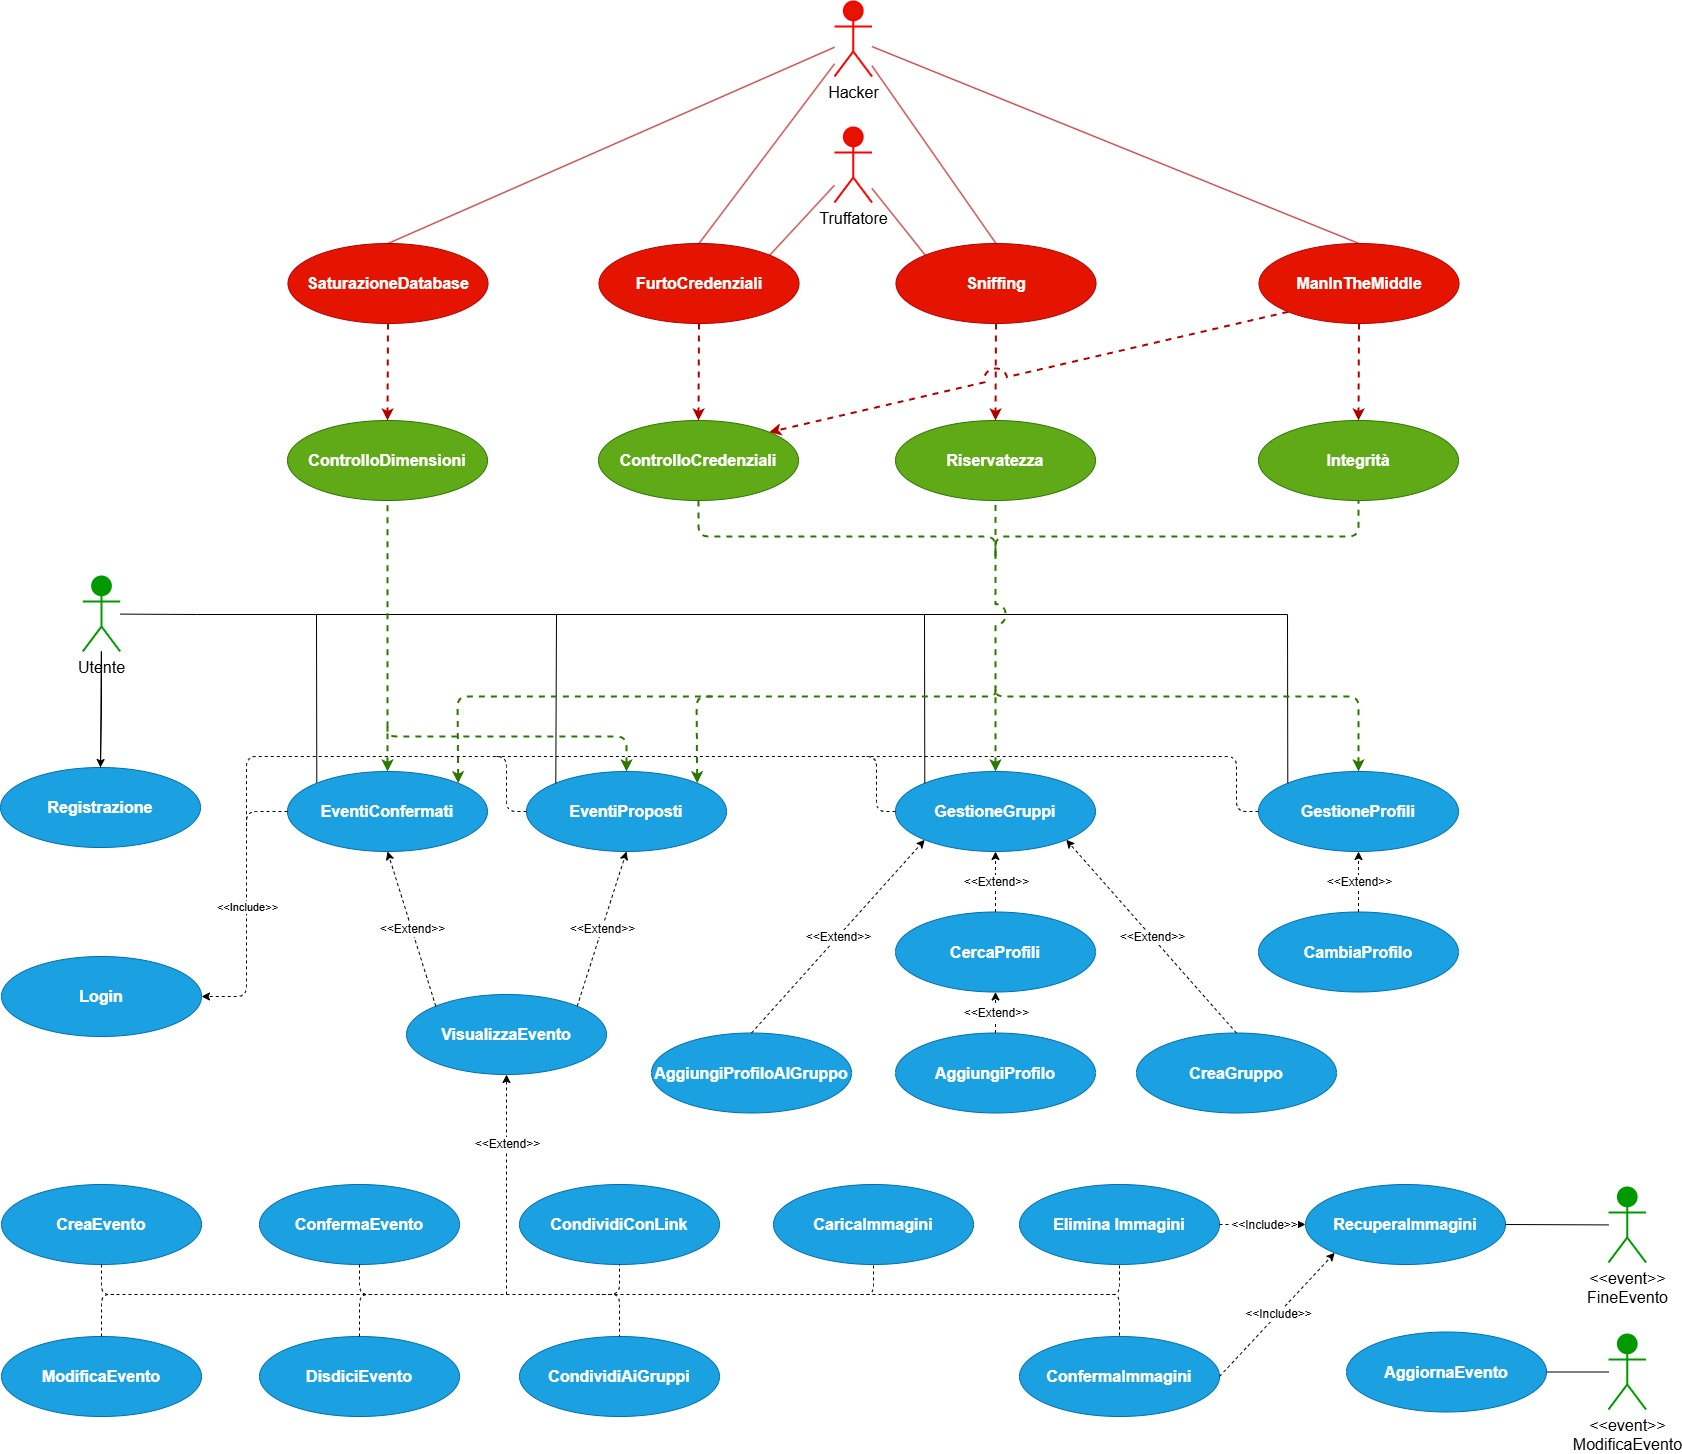
\includegraphics[width=\textwidth]{SecurityCase.jpg}
  \end{center}
\end{figure}
\newpage


\subsubsection{Security Use Case \& Misuse Case Scenari}
\hfill

%ControlloDimensioni
\begin{tabular} {|P{4cm}|P{11.5cm}|}
  \hline
  \textbf{Titolo}                                      & ControlloDimensioni                                                                          \\
  \hline
  \textbf{Descrizione}                                 & Le richieste non possono superare un una determinata dimensione                              \\
  \hline
  \textbf{Misuse case}                                 & SaturazioneDatabase                                                                          \\
  \hline
  \textbf{Relazioni}                                   &                                                                                              \\
  \hline
  \textbf{Precondizioni}                               & L'attaccante ha i mezzi per carpire grandi quantità di file                                  \\
  \hline
  \textbf{Postcondizioni}                              & Il sistema blocca la richiesta e limita la dimensione totale dei file caricati               \\
  \hline
  \textbf{Scenario principale}                         & 1. L'attaccante fa una richiesta con dimensioni molto grandi \linebreak
  2. Il sistema controlla le dimensioni della richiesta, e la blocca                                                                                  \\
  \hline
  \textbf{Scenari alternativi}                         & 1. L'attaccante fa tante richieste di salvataggio dati in un breve lasso di tempo \linebreak
  2. Il sistema controlla le dimensioni totali delle richieste per ogni lasso di tempo\linebreak
  3. Se le dimensioni totali superano il limite, ogni richiesta sucessiva viene bloccata fino allo scadere del tempo                                  \\
  \hline
  \textbf{Scenari di un attacco avvenuto con successo} & 1. L'attaccante riesce a farsi accettare le richieste con dimensioni elevate \linebreak
  2. Il sistema controlla la quantità totale di dati caricati dall'utente in un determinato lasso di tempo\linebreak
  3. Se la quantità supera il consentito, il sistema blocca l'utente                                                                                  \\
  \hline
\end{tabular}
\hfill
\break

%ControlloCredenziali
\begin{tabular} {|P{4cm}|P{11.5cm}|}
  \hline
  \textbf{Titolo}                                      & ControlloCredenziali                                            \\
  \hline
  \textbf{Descrizione}                                 & L'accesso alle funzionalità del sistema deve essere controllato \\
  \hline
  \textbf{Misuse case}                                 & FurtoCredenziali, ManInTheMiddle                                \\
  \hline
  \textbf{Relazioni}                                   &                                                                 \\
  \hline
  \textbf{Precondizioni}                               & L'attaccante ha i mezzi per carpire in tutto o in
  parte le credenziali di accesso di un utente                                                                           \\
  \hline
  \textbf{Postcondizioni}                              & Il sistema blocca l'accesso non autorizzato e
  notifica il tentativo di accesso                                                                                       \\
  \hline
  \textbf{Scenario principale}                         & 1. L'attaccante tenta di accedere al servizio
  spacciandosi per un utente legittimo, di cui conosce le credenziali solo in
  parte (ad esempio mediante attacco con dizionario) \linebreak 2. Il sistema non
  riconosce le credenziali, restituendo un errore \linebreak 3. In seguito ad un numero
  fissato di tentativi falliti, il sistema blocca temporaneamente l'accesso a
  quell'utente e notifica l'anomalia a chi di dovere                                                                     \\
  \hline
  \textbf{Scenari di un attacco avvenuto con successo} & 1. L'attaccante riesce
  a carpire le credenziali di accesso complete di un utente in un qualsiasi
  modo \linebreak 2. Il sistema riconosce la correttezza delle credenziali, e fornisce
  l'accesso al soggetto malevolo \linebreak 3. L'attaccante ha libero accesso al sistema,
  con privilegi diversi in base al tipo di utente                                                                        \\
  \hline
\end{tabular}
\hfill
\break

\begin{tabular} {|P{4cm}|P{11.5cm}|}
  \hline
  \textbf{Titolo}                                      & Riservatezza                                                    \\
  \hline
  \textbf{Descrizione}                                 & I dati non sono accessibili da chi non ne ha i permessi         \\
  \hline
  \textbf{Misuse case}                                 & Sniffing                                                        \\
  \hline
  \textbf{Relazioni}                                   &                                                                 \\
  \hline
  \textbf{Precondizioni}                               & L'attaccante ha i mezzi per intercettare i messaggi del sistema \\
  \hline
  \textbf{Postcondizioni}                              & Il sistema impedisce all'attaccante di decifrare
  (in tempi utili) i messaggi intercettati                                                                               \\
  \hline
  \textbf{Scenario principale}                         & 1. Il Sistema protegge i messaggi \linebreak
  2. L'attaccante riesce ad intercettare un messaggio \linebreak 3. L'attaccante prova
  a decifrare i messaggi, ma non riesce a trovare un modo per farlo abbastanza
  velocemente                                                                                                            \\
  \hline
  \textbf{Scenari di un attacco avvenuto con successo} & 1. Il Sistema protegge
  i messaggi \linebreak 2. L'attaccante riesce ad intercettare un messaggio \linebreak
  3. L'attaccante riesce a decifrare i messaggi e a leggerne il contenuto, ma
  solamente per una sessione di un utente                                                                                \\
  \hline
\end{tabular}
\hfill
\break

\begin{tabular} {|P{4cm}|P{11.5cm}|}
  \hline
  \textbf{Titolo}                                      & Integrità                                     \\
  \hline
  \textbf{Descrizione}                                 & Integrità dei dati del sistema                \\
  \hline
  \textbf{Misuse case}                                 & ManInTheMiddle                                \\
  \hline
  \textbf{Relazioni}                                   &                                               \\
  \hline
  \textbf{Precondizioni}                               & 1. L'attaccante ha i mezzi per intercettare i
  messaggi del sistema \linebreak 2. L'attaccante ha i mezzi per modificare i messaggi
  \linebreak 3. L'attaccante ha i mezzi per spedire il messaggio modificato al
  destinatario                                                                                         \\
  \hline
  \textbf{Postcondizioni}                              & Il sistema rileva il messaggio contraffatto   \\
  \hline
  \textbf{Scenario principale}                         & 1. Il Sistema protegge i messaggi \linebreak
  2. L'attaccante riesce ad intercettare un messaggio e lo modifica \linebreak 3. Il
  sistema si accorge del messaggio contraffatto e lo segna nei log                                     \\
  \hline
  \textbf{Scenari di un attacco avvenuto con successo} & 1. Il Sistema protegge
  i messaggi \linebreak 2. L'attaccante riesce ad intercettare un messaggio e
  lo modifica \linebreak 3. Il sistema accetta il messaggio e agisce di conseguenza,
  segnando il messaggio nei log                                                                        \\
  \hline
\end{tabular}
\hfill
\break


\subsubsection{Requisiti di Protezione dei Dati}

Sussistono inoltre i seguenti requisiti inerenti alla protezione dei dati:
\begin{enumerate}
  \item Implementare un sistema di log per tracciare tutti i messaggi tra i client e i server, inclusi gli accessi, le richieste di prenotazione, di conferma, di sospensione e di invio e ricezione di dati
  \item I dati salvati devono essere protetti da un attaccante che abbia accesso al sistema, prendendo misure di sicurezza fisica, eventualmente cifrando i dati
  \item I dati inviati tra le parti remote devono essere protetti, utilizzando la cifratura dei dati
  \item Tutte le azioni avvenute sul sistema devono essere tracciate
        tramite un sistema di log.
\end{enumerate}

\raggedright{La visione e l'analisi dei log verrà gestita
  con un editor di testo esterno, accessibile solo al personale
  autorizzato.}
\hfill \break

\begin{tabular} {|P{1.3cm}|P{11.2cm}|P{3cm}|}
  \hline
  \textbf{ID}                       & \textbf{Requisiti}                                                  & \textbf{Tipo} \\
  \hline
  R21F                              & Implementazione di un sistema di log per tracciare tutti i messaggi
  tra i client e i server           & Funzionale                                                                          \\
  \hline
  R22F                              & Le richieste non devono superare una certa dimensione               & Funzionale    \\
  \hline
  R7NF                              & I dati salvati devono essere protetti da un attaccante che abbia
  accesso al sistema, prendendo misure di sicurezza fisica, eventualmente
  cifrando i dati                   & Non Funzionale                                                                      \\
  \hline
  R8NF                              & I dati inviati tra le parti remote devono essere protetti,
  utilizzando la cifratura dei dati & Non Funzionale                                                                      \\
  \hline
\end{tabular}
